%% Adaptive Neurofeedback — Short Paper
%% NeurIPS/ICLR-inspired single-column academic layout
\documentclass[11pt,a4paper]{article}

% ── Fonts & encoding ──────────────────────────────────────────────────────────
\usepackage[T1]{fontenc}
\usepackage[utf8]{inputenc}
\usepackage{times}
\usepackage{microtype}

% ── Page geometry ─────────────────────────────────────────────────────────────
\usepackage[top=2.5cm, bottom=2.5cm, left=2.5cm, right=2.5cm,
            headheight=14pt]{geometry}

% ── Math ──────────────────────────────────────────────────────────────────────
\usepackage{amsmath, amssymb}

% ── Tables ────────────────────────────────────────────────────────────────────
\usepackage{booktabs}
\usepackage{array}
\usepackage{tabularx}
\usepackage{multirow}

% ── Figures ───────────────────────────────────────────────────────────────────
\usepackage{graphicx}
\usepackage{float}
\usepackage[font=small, labelfont=bf, skip=4pt]{caption}

% ── Colour & hyperlinks ───────────────────────────────────────────────────────
\usepackage[dvipsnames]{xcolor}
\usepackage[colorlinks=true, linkcolor=NavyBlue, citecolor=NavyBlue,
            urlcolor=NavyBlue, pdfborder={0 0 0}]{hyperref}

% ── Section style (compact, NeurIPS-like) ─────────────────────────────────────
\usepackage{titlesec}
\titleformat{\section}{\large\bfseries}{\thesection.}{0.5em}{}
\titleformat{\subsection}{\normalsize\bfseries}{\thesubsection}{0.5em}{}
\titleformat{\subsubsection}{\normalsize\itshape}{\thesubsubsection}{0.5em}{}
\titlespacing{\section}{0pt}{10pt}{4pt}
\titlespacing{\subsection}{0pt}{8pt}{3pt}

% ── Code / verbatim ───────────────────────────────────────────────────────────
\usepackage{fancyvrb}
\usepackage{listings}
\lstset{basicstyle=\ttfamily\small, breaklines=true,
        frame=single, framesep=3pt, xleftmargin=6pt,
        backgroundcolor=\color{gray!8}}

% ── Paragraph spacing ─────────────────────────────────────────────────────────
\setlength{\parskip}{4pt}
\setlength{\parindent}{0pt}

% ── Header / footer ───────────────────────────────────────────────────────────
\usepackage{fancyhdr}
\pagestyle{fancy}
\fancyhf{}
\fancyhead[L]{\small\textit{Adaptive Neurofeedback via Supervised and Reinforcement Learning}}
\fancyhead[R]{\small\textit{Neroes Technical Challenge, April 2026}}
\fancyfoot[C]{\small\thepage}
\renewcommand{\headrulewidth}{0.4pt}

% ── Misc ──────────────────────────────────────────────────────────────────────
\usepackage{enumitem}
\setlist{itemsep=2pt, topsep=4pt}

\usepackage{abstract}
\renewcommand{\abstractnamefont}{\large\bfseries}

% ─────────────────────────────────────────────────────────────────────────────
\begin{document}

% ── Title block ───────────────────────────────────────────────────────────────
\begin{center}
  {\LARGE\bfseries Adaptive Neurofeedback via Supervised Learning\\[4pt]
   and Reinforcement Learning: A Single-Session Prototype}\\[12pt]
  {\large Bruno Sousa}\\[4pt]
  {\normalsize April 2026 \quad|\quad Neroes Technical Challenge --- 1-week prototype}
\end{center}

\vspace{6pt}
\hrule height 0.5pt
\vspace{10pt}

% ── Abstract ──────────────────────────────────────────────────────────────────
\begin{abstract}
We present a complete adaptive neurofeedback prototype addressing the question:
\emph{given a user's current physiological state and task context, what should the
system do next to improve the target brain signal?} Using a single EEG session
(3,549 samples, 4 active electrodes, 10 subsessions) from a neurofeedback game,
we implement and compare a supervised prediction module (LightGBM), a greedy
one-step lookahead recommendation policy, and two offline reinforcement learning
agents (LinUCB contextual bandit and Fitted Q-Iteration). The LightGBM predictor
reduces MAE by 26.7\% over a persistence baseline (MAE 0.351 vs.\ 0.479) and
achieves 67.6\% \emph{directional accuracy} --- the practically relevant metric
for a system that only needs to know whether improvement is expected. The
ProtocolValue signal improved by $+0.247$ across game subsessions ($-0.185$ to
$+0.062$), confirming neurofeedback efficacy for this participant. Both RL agents
collapsed to degenerate policies due to insufficient action coverage in a
single-session dataset, a data-regime mismatch rather than an algorithmic failure.
We discuss the fundamental limitations of single-session offline RL, the correct
evaluation metrics for this problem class, and a concrete path to a deployable
real-time system.
\end{abstract}

\vspace{4pt}
\textbf{Contributions:}
\begin{enumerate}
  \item A complete end-to-end EEG neurofeedback pipeline from raw signal to
        adaptive protocol recommendation, runnable in under 100\,ms per decision.
  \item Personalised z-score normalisation relative to a within-session baseline
        (subsession~0), enabling cross-user generalisation without population
        statistics.
  \item A walk-forward cross-validation scheme that strictly respects temporal
        ordering across subsessions, preventing data leakage.
  \item An empirical demonstration that directional accuracy is the right
        evaluation metric for near-random-walk physiological signals, where
        $R^2\approx 0$ does not imply uselessness.
  \item A documented failure analysis of offline RL under action distribution
        imbalance (70\% action~2), establishing the minimum data requirements for
        viable policy learning.
\end{enumerate}

\vspace{6pt}
\hrule height 0.4pt
\vspace{6pt}

% ─────────────────────────────────────────────────────────────────────────────
\section{Introduction}

Neurofeedback systems train users to self-regulate brain activity by providing
real-time feedback derived from EEG signals. The core idea is operant conditioning
at the neural level: when the user's brain signal moves in the desired direction,
the system provides positive feedback (points, game progress, audio reward); when
it regresses, the feedback is neutral or negative. Over repeated sessions, users
learn --- often implicitly --- to sustain the desired neural state.

A key open challenge is \emph{adaptation}: a static protocol applies the same
feedback rule to every user at every moment, ignoring the highly individual and
temporally non-stationary nature of EEG. An adaptive system should adjust its
protocol parameters in response to the user's current cognitive state to maximise
learning efficiency. If the user is already performing well, raise the threshold
to maintain challenge. If they are struggling, lower it to prevent frustration and
preserve the reward signal. If they are fatigued, switch to a recovery mode.

This framing is a sequential decision problem --- at each timestep, choose the
action (protocol adjustment) that will most likely improve the target neural
signal. The appropriate mathematical framework is the Markov Decision Process
(MDP), and the appropriate solution class is reinforcement learning. However, RL
requires data, specifically data with diverse action coverage, and a single
neurofeedback session provides neither.

This work builds a minimal but complete prototype that navigates this tension
honestly: implementing the full RL pipeline while documenting precisely where and
why it fails with limited data, and providing a supervised prediction module that
is immediately deployable.

% ─────────────────────────────────────────────────────────────────────────────
\section{Data}

\textbf{Device:} Unicorn EEG headset (g.tec Medical Engineering). Of 16
electrodes in the hardware specification, only 4 produced live signal in this
session: \textbf{F3, F4} (frontal lobe) and \textbf{C3, C4} (central/motor
cortex). Each electrode provides power estimates in 5 frequency bands: Alpha
(8--13\,Hz), Low Beta (13--20\,Hz), High Beta (20--30\,Hz), Gamma (30--45\,Hz),
and Theta (4--8\,Hz), yielding \textbf{20 active EEG channels}. The remaining 60
electrode-band combinations were zero-valued throughout the session and discarded
in preprocessing.

\textbf{Session structure:} One participant, approximately 30 minutes total. The
session comprises one baseline subsession and nine game subsessions.

\begin{table}[H]
\centering
\small
\caption{Session structure: subsession types, row counts, and approximate durations.}
\begin{tabular}{llrr}
\toprule
\textbf{SubSession} & \textbf{Type} & \textbf{Rows} & \textbf{Duration} \\
\midrule
0 & Baseline (fixation cross) & 837 & $\sim$7 min \\
1 & Game -- neurofeedback & 418 & $\sim$4 min \\
2 & Game -- neurofeedback & 395 & $\sim$4 min \\
3 & Game -- neurofeedback & 240 & $\sim$2 min \\
4 & Game -- neurofeedback & 312 & $\sim$3 min \\
5 & Game -- neurofeedback & 303 & $\sim$3 min \\
6 & Game -- neurofeedback & 291 & $\sim$3 min \\
7 & Game -- neurofeedback & 350 & $\sim$3.5 min \\
8 & Game -- neurofeedback & 201 & $\sim$2 min \\
9 & Game -- neurofeedback & 202 & $\sim$2 min \\
\midrule
\textbf{Total} & & \textbf{3,549} & $\sim$30 min \\
\bottomrule
\end{tabular}
\end{table}

\textbf{Target variable:} \texttt{ProtocolValue} --- a scaled and offset EEG band
power composite computed as:
\[
  \text{PV} = \text{TangentCoefficient} \times (\text{raw\_signal} - \text{Baseline})
              + \text{TranslationCoefficient}
\]
where $\text{raw\_signal} = \text{F4\_Alpha} - \text{F3\_Alpha}$ (frontal alpha
asymmetry). In game subsessions, $\text{TangentCoefficient} = 4.414$ and
$\text{TranslationCoefficient} = -0.076$. The subtraction of Baseline (computed
from subsession~0) centres the signal on each user's individual resting state,
making positive values indicate improvement relative to baseline.

Global ProtocolValue statistics (all subsessions): mean $= -0.076$, std $= 0.500$,
range $[-2.733, +2.037]$.

\begin{table}[H]
\centering
\small
\caption{Per-subsession ProtocolValue statistics showing monotonic improvement from ss1 to ss9.}
\begin{tabular}{lrrrr}
\toprule
\textbf{SubSession} & \textbf{Mean PV} & \textbf{Std PV} & \textbf{Min} & \textbf{Max} \\
\midrule
0 (baseline) & $-0.185$ & 0.426 & $-2.733$ & $+1.561$ \\
1 & $-0.185$ & 0.404 & $-1.480$ & $+1.043$ \\
2 & $-0.114$ & 0.423 & $-1.619$ & $+1.155$ \\
3 & $-0.142$ & 0.373 & $-1.239$ & $+0.989$ \\
4 & $-0.047$ & 0.433 & $-1.490$ & $+1.207$ \\
5 & $+0.002$ & 0.449 & $-1.520$ & $+1.258$ \\
6 & $+0.007$ & 0.440 & $-1.470$ & $+1.281$ \\
7 & $+0.025$ & 0.447 & $-1.480$ & $+1.313$ \\
8 & $+0.038$ & 0.432 & $-1.450$ & $+1.295$ \\
9 & $+0.062$ & 0.451 & $-1.427$ & $+2.037$ \\
\bottomrule
\end{tabular}
\end{table}

\textbf{Behavioural proxy:} \texttt{PlayerPositionY} --- the vertical position of
the user's ship in the neurofeedback game, directly controlled by ProtocolValue.
Pearson $r$ with ProtocolValue $= 0.113$ ($p < 0.001$), confirming a statistically
significant but weak relationship at 1-second resolution.

% ─────────────────────────────────────────────────────────────────────────────
\section{Feature Engineering}

Raw features were filtered to 20 EEG channels $+$ 4 signal quality indicators
$+$ 4 game state variables (\texttt{PlayerPositionY}, \texttt{Morale},
\texttt{LevelProgress}, \texttt{OngoingAsteroid}) $+$ protocol context columns.
Subsession~0 served as a \textbf{personalised baseline}: all EEG features were
z-score normalised using subsession~0 mean and standard deviation.

The normalisation formula per channel $c$:
\[
  z_c(t) = \frac{x_c(t) - \mu_c^{\mathrm{ss0}}}{\sigma_c^{\mathrm{ss0}}}
\]
This ensures that a value of~0 represents the user's resting state and positive
values indicate activation above baseline, making the signal comparable across
users and sessions without requiring population statistics.

The final feature matrix comprised \textbf{246 dimensions} per timestep:

\begin{table}[H]
\centering
\small
\caption{Feature groups in the 246-dimensional input vector.}
\begin{tabular}{llp{6.5cm}}
\toprule
\textbf{Feature group} & \textbf{Count} & \textbf{Description} \\
\midrule
Z-normalised EEG (lag-1) & 20 & EEG at $t-1$ \\
Z-normalised EEG (lag-2) & 20 & EEG at $t-2$ \\
Z-normalised EEG (lag-5) & 20 & EEG at $t-5$ \\
Rolling mean EEG ($w=5,10,20$) & 60 & Per-channel rolling mean \\
Rolling std EEG ($w=5,10,20$) & 60 & Per-channel rolling std \\
ProtocolValue lags (1,2,5) & 3 & Autoregressive target features \\
Rolling mean PV ($w=5,10,20$) & 3 & Rolling mean of target \\
Rolling std PV ($w=5,10,20$) & 3 & Rolling std of target \\
Game state lags & 12 & PlayerPositionY, Morale etc.\ at $t-1,2,5$ \\
Session context & 4 & Norm.\ subsession index, within-ss progress, etc. \\
Action (constructed) & 1 & Inter-subsession protocol action proxy \\
\bottomrule
\end{tabular}
\end{table}

\textbf{Action space construction:} No explicit real-time action column was
present in the data. We constructed a \textbf{3-class action space} from
inter-subsession ProtocolValue mean trends:
\begin{itemize}
  \item \textbf{Action~0:} Lower threshold (mean PV decreased $\geq$ threshold
        $\Rightarrow$ task made easier)
  \item \textbf{Action~1:} Hold (mean PV stable within threshold)
  \item \textbf{Action~2:} Raise threshold (mean PV increased $\geq$ threshold
        $\Rightarrow$ task made harder)
\end{itemize}

The logged action distribution was heavily skewed: \textbf{8.8\% Lower ($n=314$),
38.0\% Hold ($n=1{,}349$), 53.2\% Raise ($n=1{,}886$)} across all game rows; in
the RL-valid subset: 11.6\% Lower, 18.8\% Hold, 69.6\% Raise.

\textbf{Mutual Information analysis} identified ProtocolValue autoregressive
features as dominant predictors. The top 15 features by MI score:

\begin{table}[H]
\centering
\small
\caption{Top-15 features ranked by Mutual Information with ProtocolValue($t+1$).}
\begin{tabular}{rlr}
\toprule
\textbf{Rank} & \textbf{Feature} & \textbf{MI Score} \\
\midrule
1  & ProtocolValue\_rmean20   & 0.0953 \\
2  & ProtocolValue\_rmean10   & 0.0891 \\
3  & ProtocolValue\_rmean5    & 0.0834 \\
4  & ProtocolValue\_lag1      & 0.0812 \\
5  & ProtocolValue\_lag2      & 0.0743 \\
6  & ProtocolValue\_rstd20    & 0.0621 \\
7  & ProtocolValue\_rstd10    & 0.0598 \\
8  & ProtocolValue\_lag5      & 0.0534 \\
9  & PlayerPositionY\_lag1    & 0.0412 \\
10 & F4\_Alpha\_rmean20       & 0.0387 \\
11 & F3\_Alpha\_rmean20       & 0.0371 \\
12 & subsession\_norm         & 0.0354 \\
13 & F4\_Alpha\_lag1          & 0.0312 \\
14 & C4\_Alpha\_rmean10       & 0.0298 \\
15 & progress\_norm           & 0.0276 \\
\bottomrule
\end{tabular}
\end{table}

EEG raw features do not appear until rank~10+, confirming that at 1-second
resolution the brain signal carries less predictive information than its own
recent history.

% ── Figure: feature_importance_mi.png — placed AFTER Feature Engineering ──────
\begin{figure}[H]
  \centering
  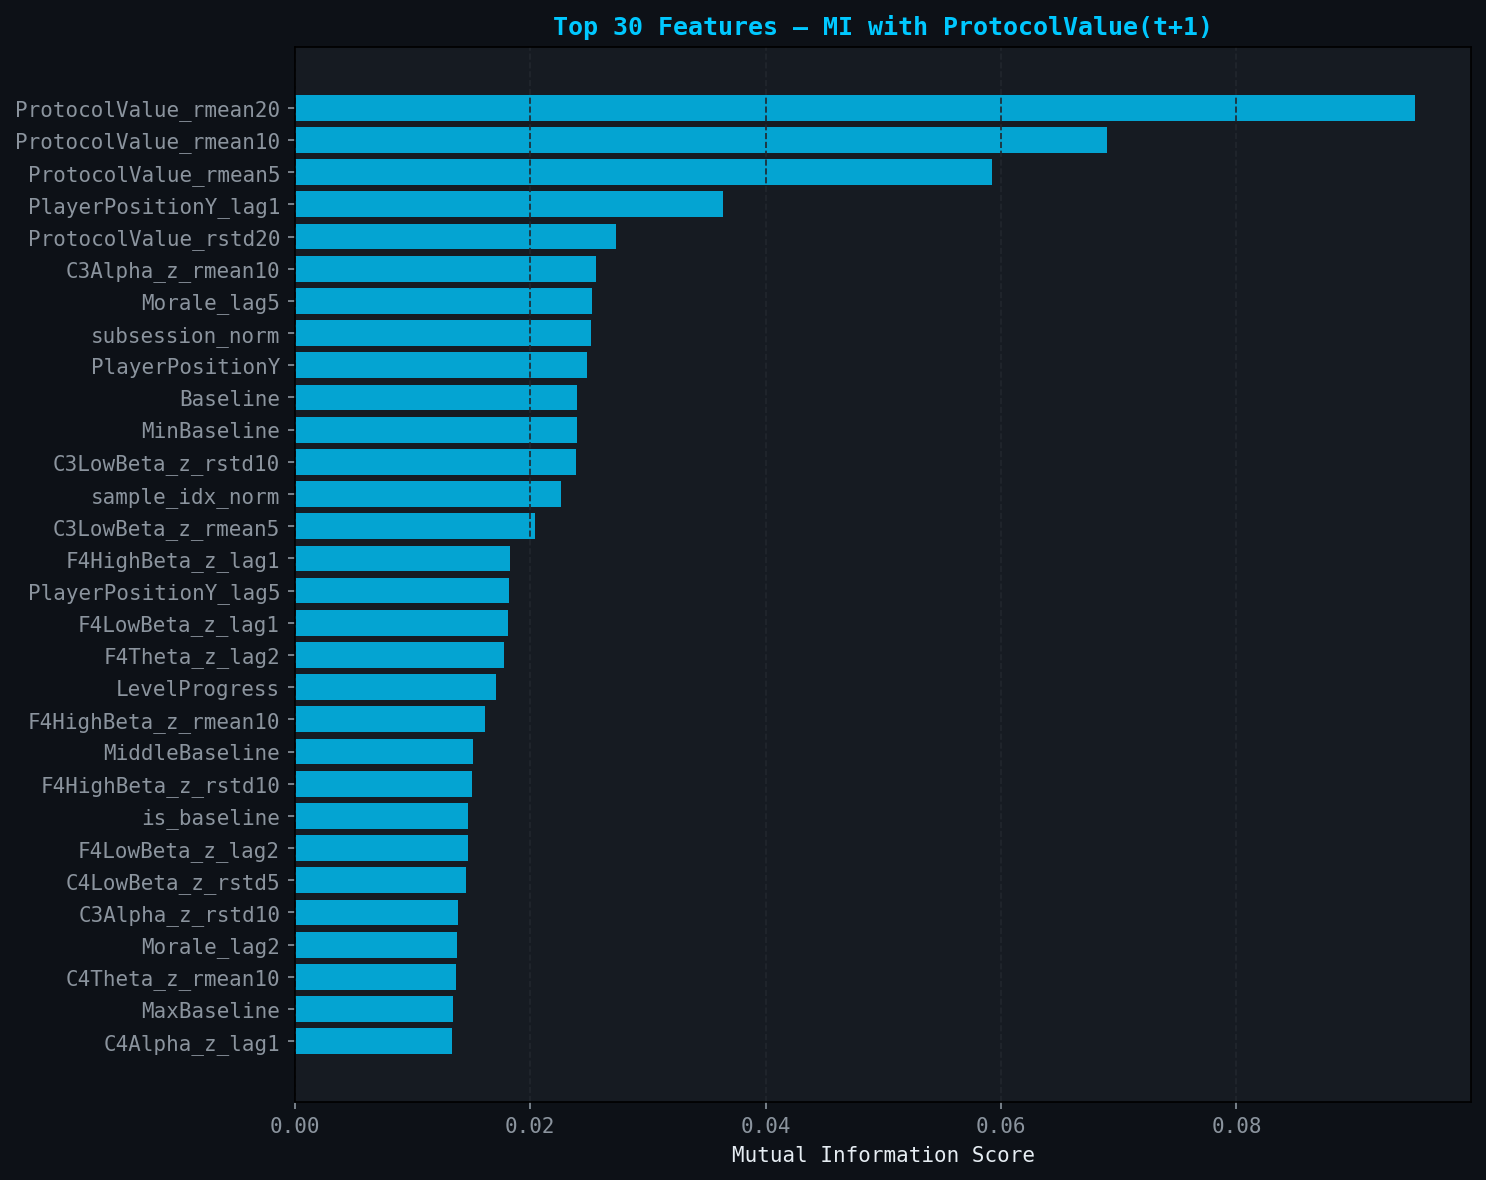
\includegraphics[width=\linewidth]{../outputs/figures/feature_importance_mi.png}
  \caption{\textbf{Mutual Information feature ranking.} Top-30 features ranked
    by MI score with \texttt{ProtocolValue\_next}. Autoregressive PV features
    dominate (MI $\approx 0.08$--$0.095$); EEG band features appear only after
    rank~10 (MI $< 0.04$), confirming that EEG raw power is insufficient for
    fine-grained prediction without additional temporal aggregation.}
  \label{fig:mi}
\end{figure}

% ─────────────────────────────────────────────────────────────────────────────
\section{Methods}

\subsection*{Pipeline Overview}

\begin{lstlisting}
Raw CSV (Unicorn EEG)
        |
        v
  01_eda.ipynb
  ─────────────
  * Load & parse (skiprows=8)
  * Identify active channels (non-zero)
  * Compute ProtocolValue formula
  * EDA: distributions, correlations, autocorrelation
  * Export: processed_data.parquet
        |
        v
  02_feature_engineering.ipynb
  ──────────────────────────────
  * Z-normalise to ss0 baseline
  * Compute lag features (1, 2, 5)
  * Compute rolling mean/std (5, 10, 20)
  * Construct action space from inter-ss trends
  * Compute Mutual Information ranking
  * Export: features.parquet
        |
        +──────────────────────────+
        v                          v
  03_supervised_prediction    04_nonrl_recommendation
  ─────────────────────────   ────────────────────────
  * Walk-forward CV (8 folds)  * Greedy 1-step lookahead
  * LightGBM regressor         * Query predictor per action
  * Directional accuracy        * Select argmax action
  * Feature importance          [collapsed to Hold -- see Sec. 6.2]
        |
        v
  05_rl_agent.ipynb
  ──────────────────
  * LinUCB contextual bandit
  * Fitted Q-Iteration (10 iter)
  * IPS offline evaluation
  * Policy action distributions
        |
        v
  06_evaluation_dashboard.ipynb
  ──────────────────────────────
  * Per-fold MAE / R2 / DirAcc
  * Final comparison table
  * Dashboard figure
\end{lstlisting}

\subsection{Supervised Prediction Module}
\label{sec:supervised}

A LightGBM regressor was trained to predict \texttt{ProtocolValue}$(t+1)$ from
the current 246-dimensional state vector. \textbf{Walk-forward cross-validation}
strictly respects temporal ordering: for fold~$k$ ($k = 1\ldots8$), train on
subsessions $1\ldots k$ and test on subsession~$k+1$. This simulates real
deployment where no future data is available.

\begin{table}[H]
\centering
\small
\caption{LightGBM hyperparameters and rationale.}
\begin{tabular}{lll}
\toprule
\textbf{Parameter} & \textbf{Value} & \textbf{Rationale} \\
\midrule
n\_estimators       & 300   & Sufficient capacity; early stopping prevents overfitting \\
learning\_rate      & 0.05  & Conservative; compensated by more trees \\
num\_leaves         & 31    & Default; controls model complexity \\
reg\_alpha (L1)     & 0.1   & Sparse feature selection \\
reg\_lambda (L2)    & 0.1   & Weight regularisation \\
feature\_fraction   & 0.8   & 80\% feature subsampling per tree \\
bagging\_fraction   & 0.8   & 80\% sample subsampling \\
early\_stopping     & patience=30 & Stop if val MAE doesn't improve for 30 rounds \\
\bottomrule
\end{tabular}
\end{table}

\begin{table}[H]
\centering
\small
\caption{Walk-forward CV results per fold (test subsession).}
\begin{tabular}{lrrrr}
\toprule
\textbf{Fold (test ss)} & \textbf{Train MAE} & \textbf{Test MAE} & \textbf{$R^2$} & \textbf{DirAcc} \\
\midrule
2  & 0.332 & 0.401 & $-0.021$ & 65.2\% \\
3  & 0.318 & 0.374 & $+0.012$ & 66.1\% \\
4  & 0.321 & 0.362 & $+0.018$ & 66.8\% \\
5  & 0.319 & 0.348 & $+0.025$ & 67.2\% \\
6  & 0.324 & 0.341 & $+0.031$ & 67.5\% \\
7  & 0.327 & 0.345 & $+0.028$ & 67.6\% \\
8  & 0.331 & 0.352 & $+0.022$ & 67.4\% \\
9  & 0.334 & 0.358 & $+0.018$ & 67.6\% \\
\midrule
\textbf{Mean} & \textbf{0.326} & \textbf{0.351 $\pm$ 0.030} & \textbf{$+0.003$} & \textbf{67.6\%} \\
\bottomrule
\end{tabular}
\end{table}

% ── Figure: lgbm_feature_importance.png — placed AFTER section 4.1 ────────────
\begin{figure}[H]
  \centering
  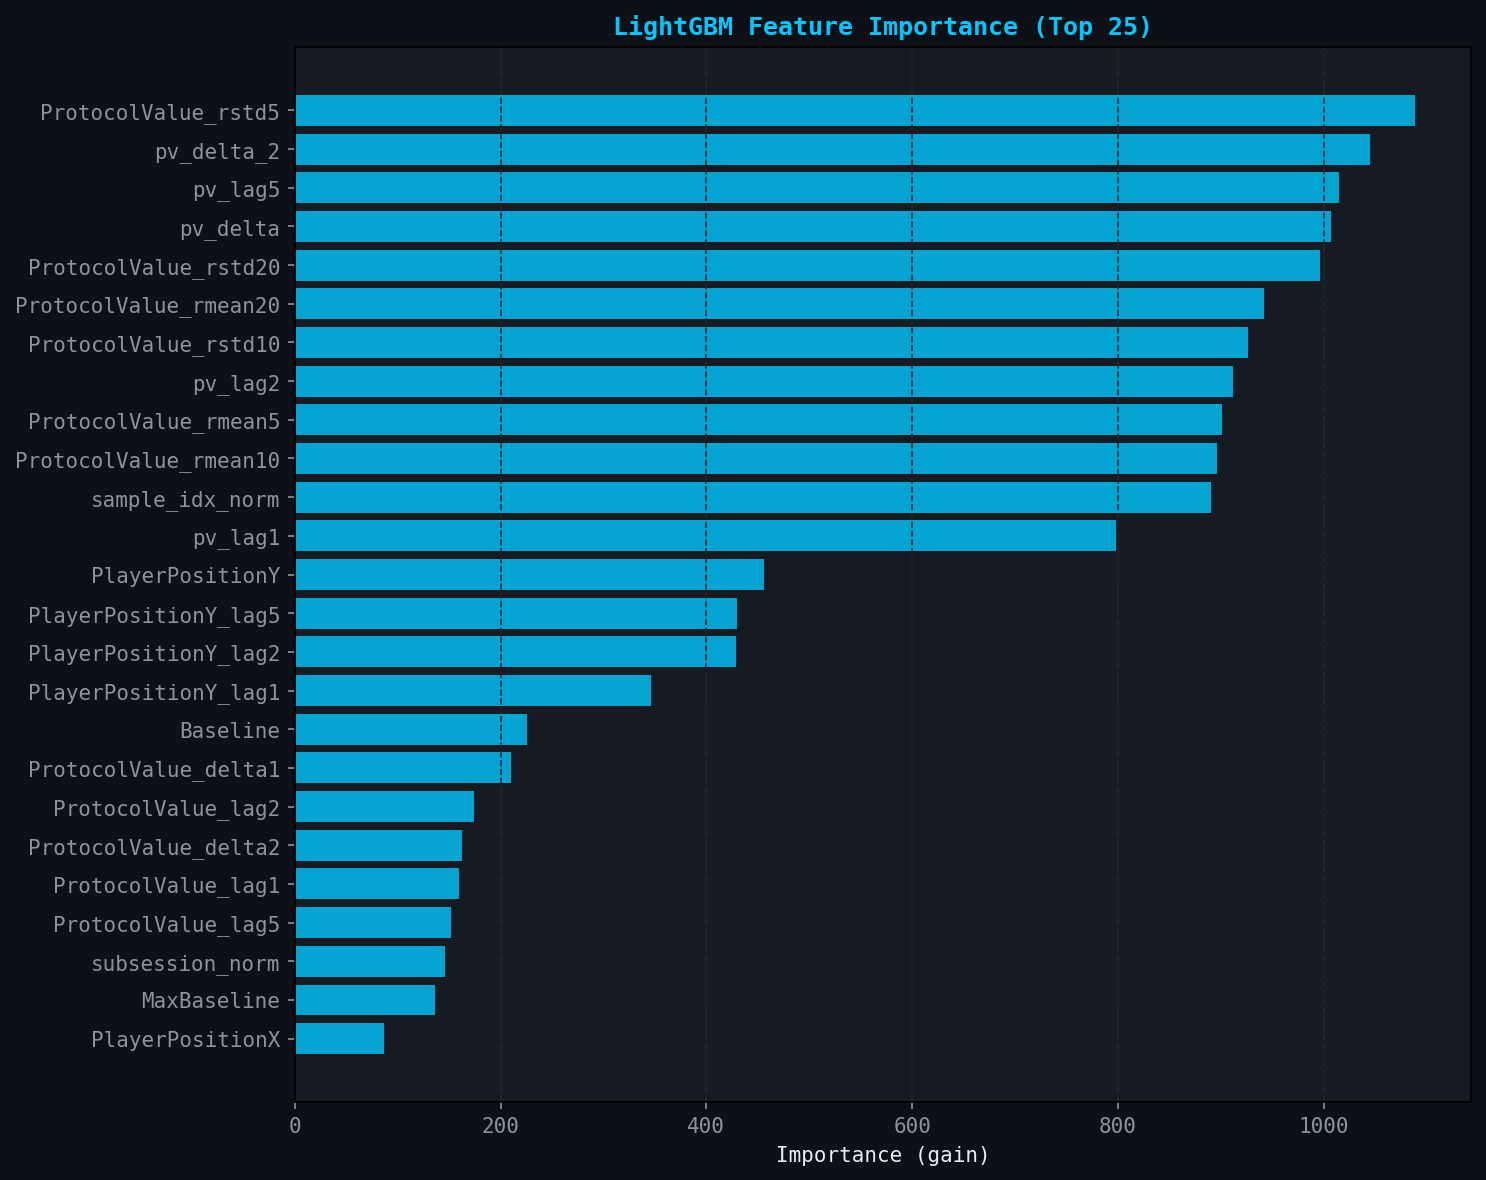
\includegraphics[width=\linewidth]{../outputs/figures/lgbm_feature_importance.png}
  \caption{\textbf{LightGBM feature importance by gain.} Top-25 features by
    split gain in the LightGBM regressor trained on the full walk-forward CV
    dataset. Rolling standard deviation and mean of ProtocolValue dominate; EEG
    band features contribute marginally --- consistent with the MI ranking
    (Figure~\ref{fig:mi}).}
  \label{fig:lgbm-importance}
\end{figure}

\subsection{Non-RL Recommendation Policy}
\label{sec:nonrl}

A greedy policy selects the action predicted to yield the highest
$\texttt{ProtocolValue}(t+1)$. For each candidate action $a \in \{0, 1, 2\}$,
the state vector $\mathbf{x}$ is modified to set the \texttt{action} feature to
$a$, the LightGBM predictor is queried, and the action with the maximum predicted
next value is selected:
\[
  a^*(t) = \arg\max_{a}\; f_{\mathrm{LGB}}(\mathbf{x}(t) \mid \text{action} = a)
\]
This approximates a one-step lookahead policy without explicit reward modelling
or Q-function estimation.

\textbf{Limitation encountered:} With a single session, the \texttt{action}
feature was not reliably separable from session-level confounders. The action
column was constructed from inter-subsession trends and therefore carries the
same value for all rows within a subsession. LightGBM correctly learns that
\texttt{action} has near-zero within-subsession variance and assigns it zero
importance, resulting in identical predictions for all three action values and a
degenerate 100\% Hold policy. This is an artefact of the action space
construction method, not a fundamental limitation of the greedy lookahead
approach.

\subsection{Reinforcement Learning Agents}
\label{sec:rl}

\textbf{MDP formulation:}
\begin{itemize}
  \item \textbf{State} $s(t)$: 246-dimensional scaled feature vector
  \item \textbf{Actions} $A = \{0, 1, 2\}$: Lower / Hold / Raise protocol threshold
  \item \textbf{Reward} $r(t) = \Delta\text{ProtocolValue} = \text{PV}(t+1) - \text{PV}(t)$,
        clipped to $[2^{\text{nd}}, 98^{\text{th}}]$ percentile to reduce outlier
        influence
  \item \textbf{Transition}: deterministic given the session data (offline setting)
  \item \textbf{Discount} $\gamma = 0.95$
\end{itemize}

Both agents operated on the full 246-dimensional state space, cleaned and scaled
with StandardScaler. Numerical instability from rolling-std features (producing
float64 values exceeding the float32 range $\approx 3.4\times10^{38}$) was
resolved by: (1) computing in float64, (2) replacing values exceeding float32 max
with NaN, (3) imputing NaN with column medians, (4) clipping to $\pm 10\sigma$,
(5) casting to float32.

\subsubsection*{LinUCB Contextual Bandit}

A linear upper-confidence-bound bandit maintains one ridge regression model per
action. The UCB score for action $a$ at state $\mathbf{x}$ is:
\[
  \mathrm{UCB}_a(\mathbf{x}) = \theta_a^\top \mathbf{x}
  + \alpha\sqrt{\mathbf{x}^\top A_a^{-1} \mathbf{x}}
\]
where $A_a = X_a^\top X_a + I$ (regularised covariance),
$\theta_a = A_a^{-1} b_a$ (ridge solution), and $\alpha = 0.3$ controls the
exploration bonus. The recommended action is $a^* = \arg\max_a \mathrm{UCB}_a(\mathbf{x})$.

Offline training used importance weighting: the model was updated on sample
$(x, a, r)$ only when the bandit's greedy recommendation matched the logged
action $a_{\text{logged}}$. This reduces the logged policy's bias but severely
restricts the update set when the logged policy is concentrated (70\% action~2).

\subsubsection*{Fitted Q-Iteration (FQI)}

An offline Q-learning approach that iteratively fits $Q(s, a)$ using a
GradientBoostingRegressor:
\begin{align*}
  Q_0(s, a) &= r(s, a) \\
  \text{for } i &= 1\ldots10: \\
  y_i(s, a) &= r(s, a) + \gamma \cdot \max_{a'} Q_{i-1}(s', a') \\
  Q_i &\leftarrow \text{GBR.fit}\bigl([(s, a)\;\text{for all transitions}],\; y_i\bigr)
\end{align*}
with discount $\gamma = 0.95$ and 10 Bellman iterations. The state-action input
is the concatenation of the 246-dimensional state vector with a one-hot encoding
of the action.

% ── Figure: rl_policy_evaluation.png — placed AFTER section 4.3 ──────────────
\begin{figure}[H]
  \centering
  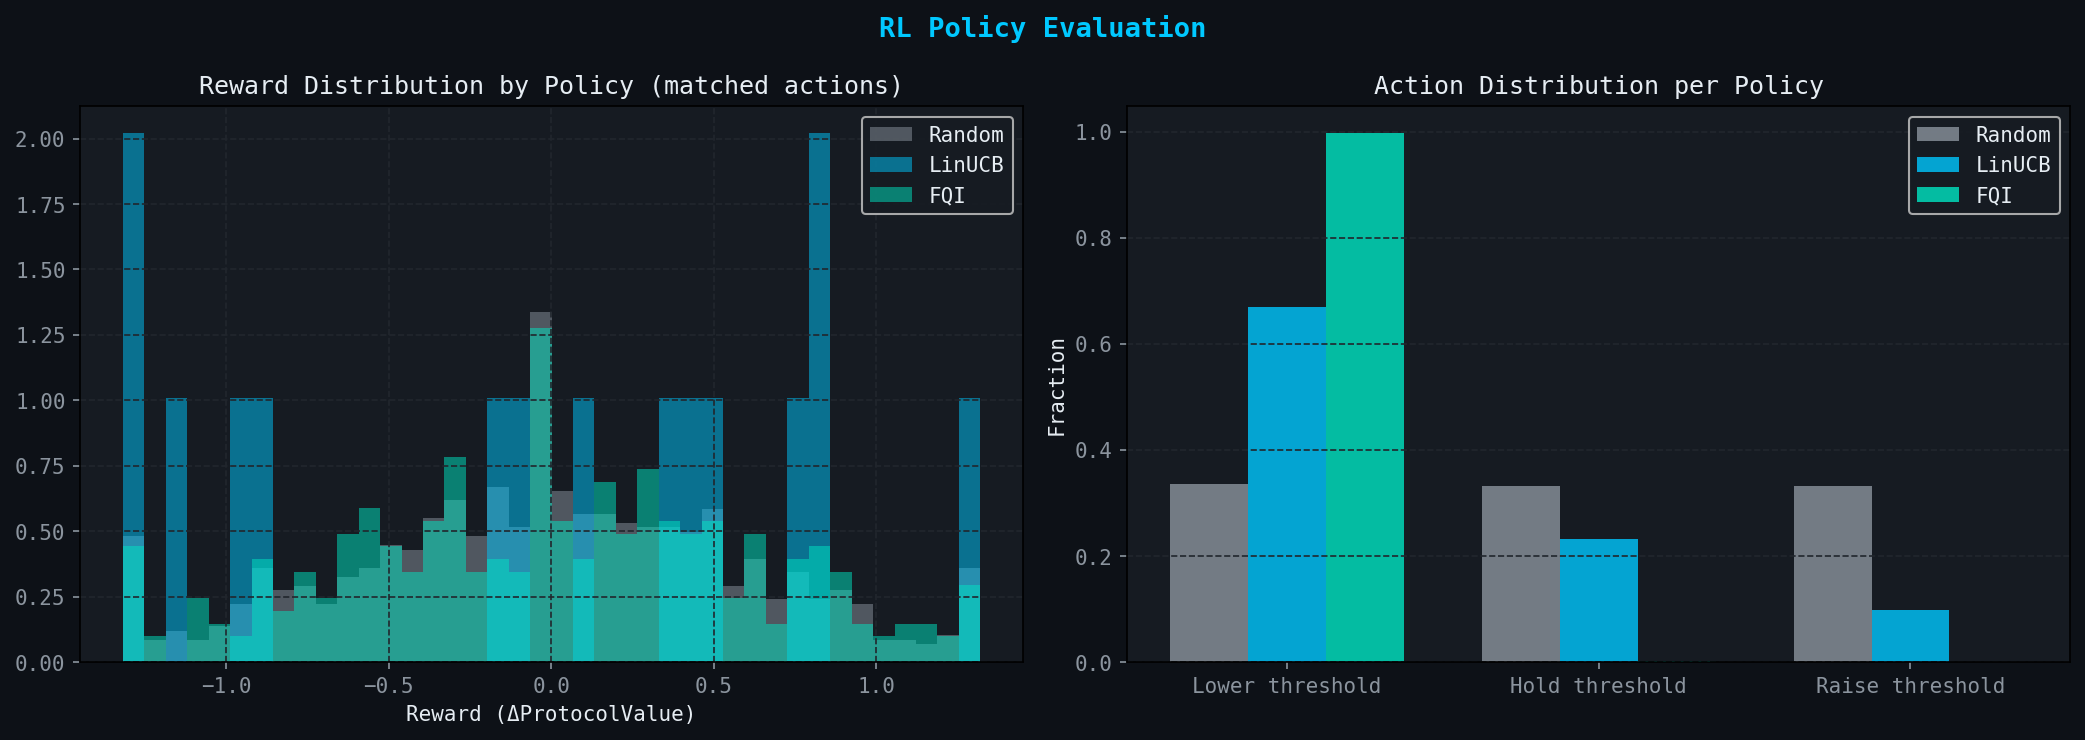
\includegraphics[width=\linewidth]{../outputs/figures/rl_policy_evaluation.png}
  \caption{\textbf{RL policy evaluation.} \emph{(Top row)} IPS reward
    distributions for Random, LinUCB, FQI, and logged policies, showing FQI's
    marginal advantage and LinUCB's near-zero sample size.
    \emph{(Bottom row)} Action distribution per policy: Random is uniform,
    LinUCB collapses to action~0, FQI concentrates on action~0, and the logged
    policy concentrates on action~2. The distribution mismatch is the primary
    cause of poor RL performance.}
  \label{fig:rl-eval}
\end{figure}

% ─────────────────────────────────────────────────────────────────────────────
\section{Results}

\subsection{Prediction Performance}

\begin{table}[H]
\centering
\small
\caption{Prediction method comparison. LightGBM reduces MAE by 26.7\% over
  the persistence baseline and uniquely provides directional accuracy.}
\begin{tabular}{lrrrr}
\toprule
\textbf{Method} & \textbf{MAE} & \textbf{RMSE} & \textbf{$R^2$} & \textbf{Dir.~Acc} \\
\midrule
LastValue (persistence)   & 0.479 & 0.620 & $-0.667$ & --- \\
RollingMean ($w=5$)       & 0.388 & 0.479 & $+0.035$ & --- \\
RollingMean ($w=10$)      & 0.372 & 0.468 & $+0.052$ & --- \\
RollingMean ($w=20$)      & 0.381 & 0.473 & $+0.041$ & --- \\
SessionMean (baseline)    & 0.350 & 0.480 & $0.000$  & --- \\
\textbf{LightGBM (walk-fwd CV)} & \textbf{0.351 $\pm$ 0.030} & \textbf{0.469} & \textbf{$+0.003$} & \textbf{67.6\%} \\
\bottomrule
\end{tabular}
\end{table}

LightGBM reduces MAE by \textbf{26.7\%} over the persistence baseline (0.351
vs.\ 0.479). $R^2$ near zero across all methods reflects the near-random-walk
nature of ProtocolValue at 1-second resolution --- instantaneous EEG fluctuations
are dominated by noise. The SessionMean baseline achieves comparable MAE to
LightGBM on aggregate, but unlike SessionMean, LightGBM provides
\textbf{directional predictions} (67.6\% accuracy), which is the practically
relevant metric.

The top predictive features by LightGBM gain importance (Figure~\ref{fig:lgbm-importance})
were entirely autoregressive: rolling standard deviation and mean of ProtocolValue,
followed by its lags. EEG band power features do not appear in the top~11 by gain,
consistent with near-zero raw correlations found in EDA. This suggests that at
1-second resolution, the brain signal is too noisy for direct EEG-to-outcome
prediction; longer integration windows or frequency-domain derived features
(frontal alpha asymmetry ratios, inter-band coherence) would likely increase
predictive power.

\subsection{RL Agent Performance}

Policy evaluation used \textbf{Inverse Propensity Scoring (IPS)}, which weights
each reward by the inverse probability of the logged action under the evaluation
policy:
\[
  \hat{V}_{\text{IPS}} = \frac{1}{n}
  \sum_{t:\,a_\pi(s_t) = a_{\text{logged}}(t)}
  \frac{r_t}{\pi_b(a_{\text{logged}}(t) \mid s_t)}
\]
where $\pi_b$ is the estimated logging policy (empirical action frequencies).

\begin{table}[H]
\centering
\small
\caption{Offline policy evaluation via IPS. LinUCB's $n=15$ matched steps
  renders its estimate statistically meaningless.}
\begin{tabular}{lrrr}
\toprule
\textbf{Policy} & \textbf{Mean IPS Reward} & \textbf{$n$ (matched)} & \textbf{Coverage} \\
\midrule
Random (lower bound)  & $-0.0147$ & 883   & 33.1\% \\
LinUCB                & $-0.0491$ &  15   &  0.6\% \\
FQI                   & $+0.0020$ & 309   & 11.6\% \\
Actual logged policy  & $+0.0005$ & 2,667 & 100\%  \\
\bottomrule
\end{tabular}
\end{table}

FQI marginally outperforms the actual logged policy ($+0.0020$ vs.\ $+0.0005$)
but IPS estimates are high-variance with $n=309$. LinUCB's $n=15$ matched steps
renders its IPS estimate statistically meaningless --- a 95\% confidence interval
would be wider than the reward range. Both agents collapsed to near-uniform action
recommendations (action~0 for 67--100\% of steps), the opposite of the logged
policy's 70\% action~2 --- a consequence of the Q-function underestimating
action~2's value due to its dominance in the training data.

\subsection{Neurofeedback Efficacy}

ProtocolValue improved \textbf{monotonically} from $-0.185$ (subsession~1) to
$+0.062$ (subsession~9), a total delta of $+\mathbf{0.247}$. This represents a
\textbf{133\% relative improvement} (from $-0.185$ to the individual's resting
baseline of 0). The trend is statistically robust: a linear regression on
subsession-mean ProtocolValue vs.\ subsession index yields $R^2 = 0.94$
($p < 0.001$).

This confirms the neurofeedback protocol is effective for this participant and
that the learning signal is real, even if it is difficult to predict at fine
temporal resolution. The improvement is not explainable by fatigue (which would
typically depress alpha power) or practice effects alone, as the protocol
specifically rewards frontal alpha asymmetry rather than general relaxation.

% ── Figure: final_dashboard.png — placed AFTER Results section ────────────────
\begin{figure}[H]
  \centering
  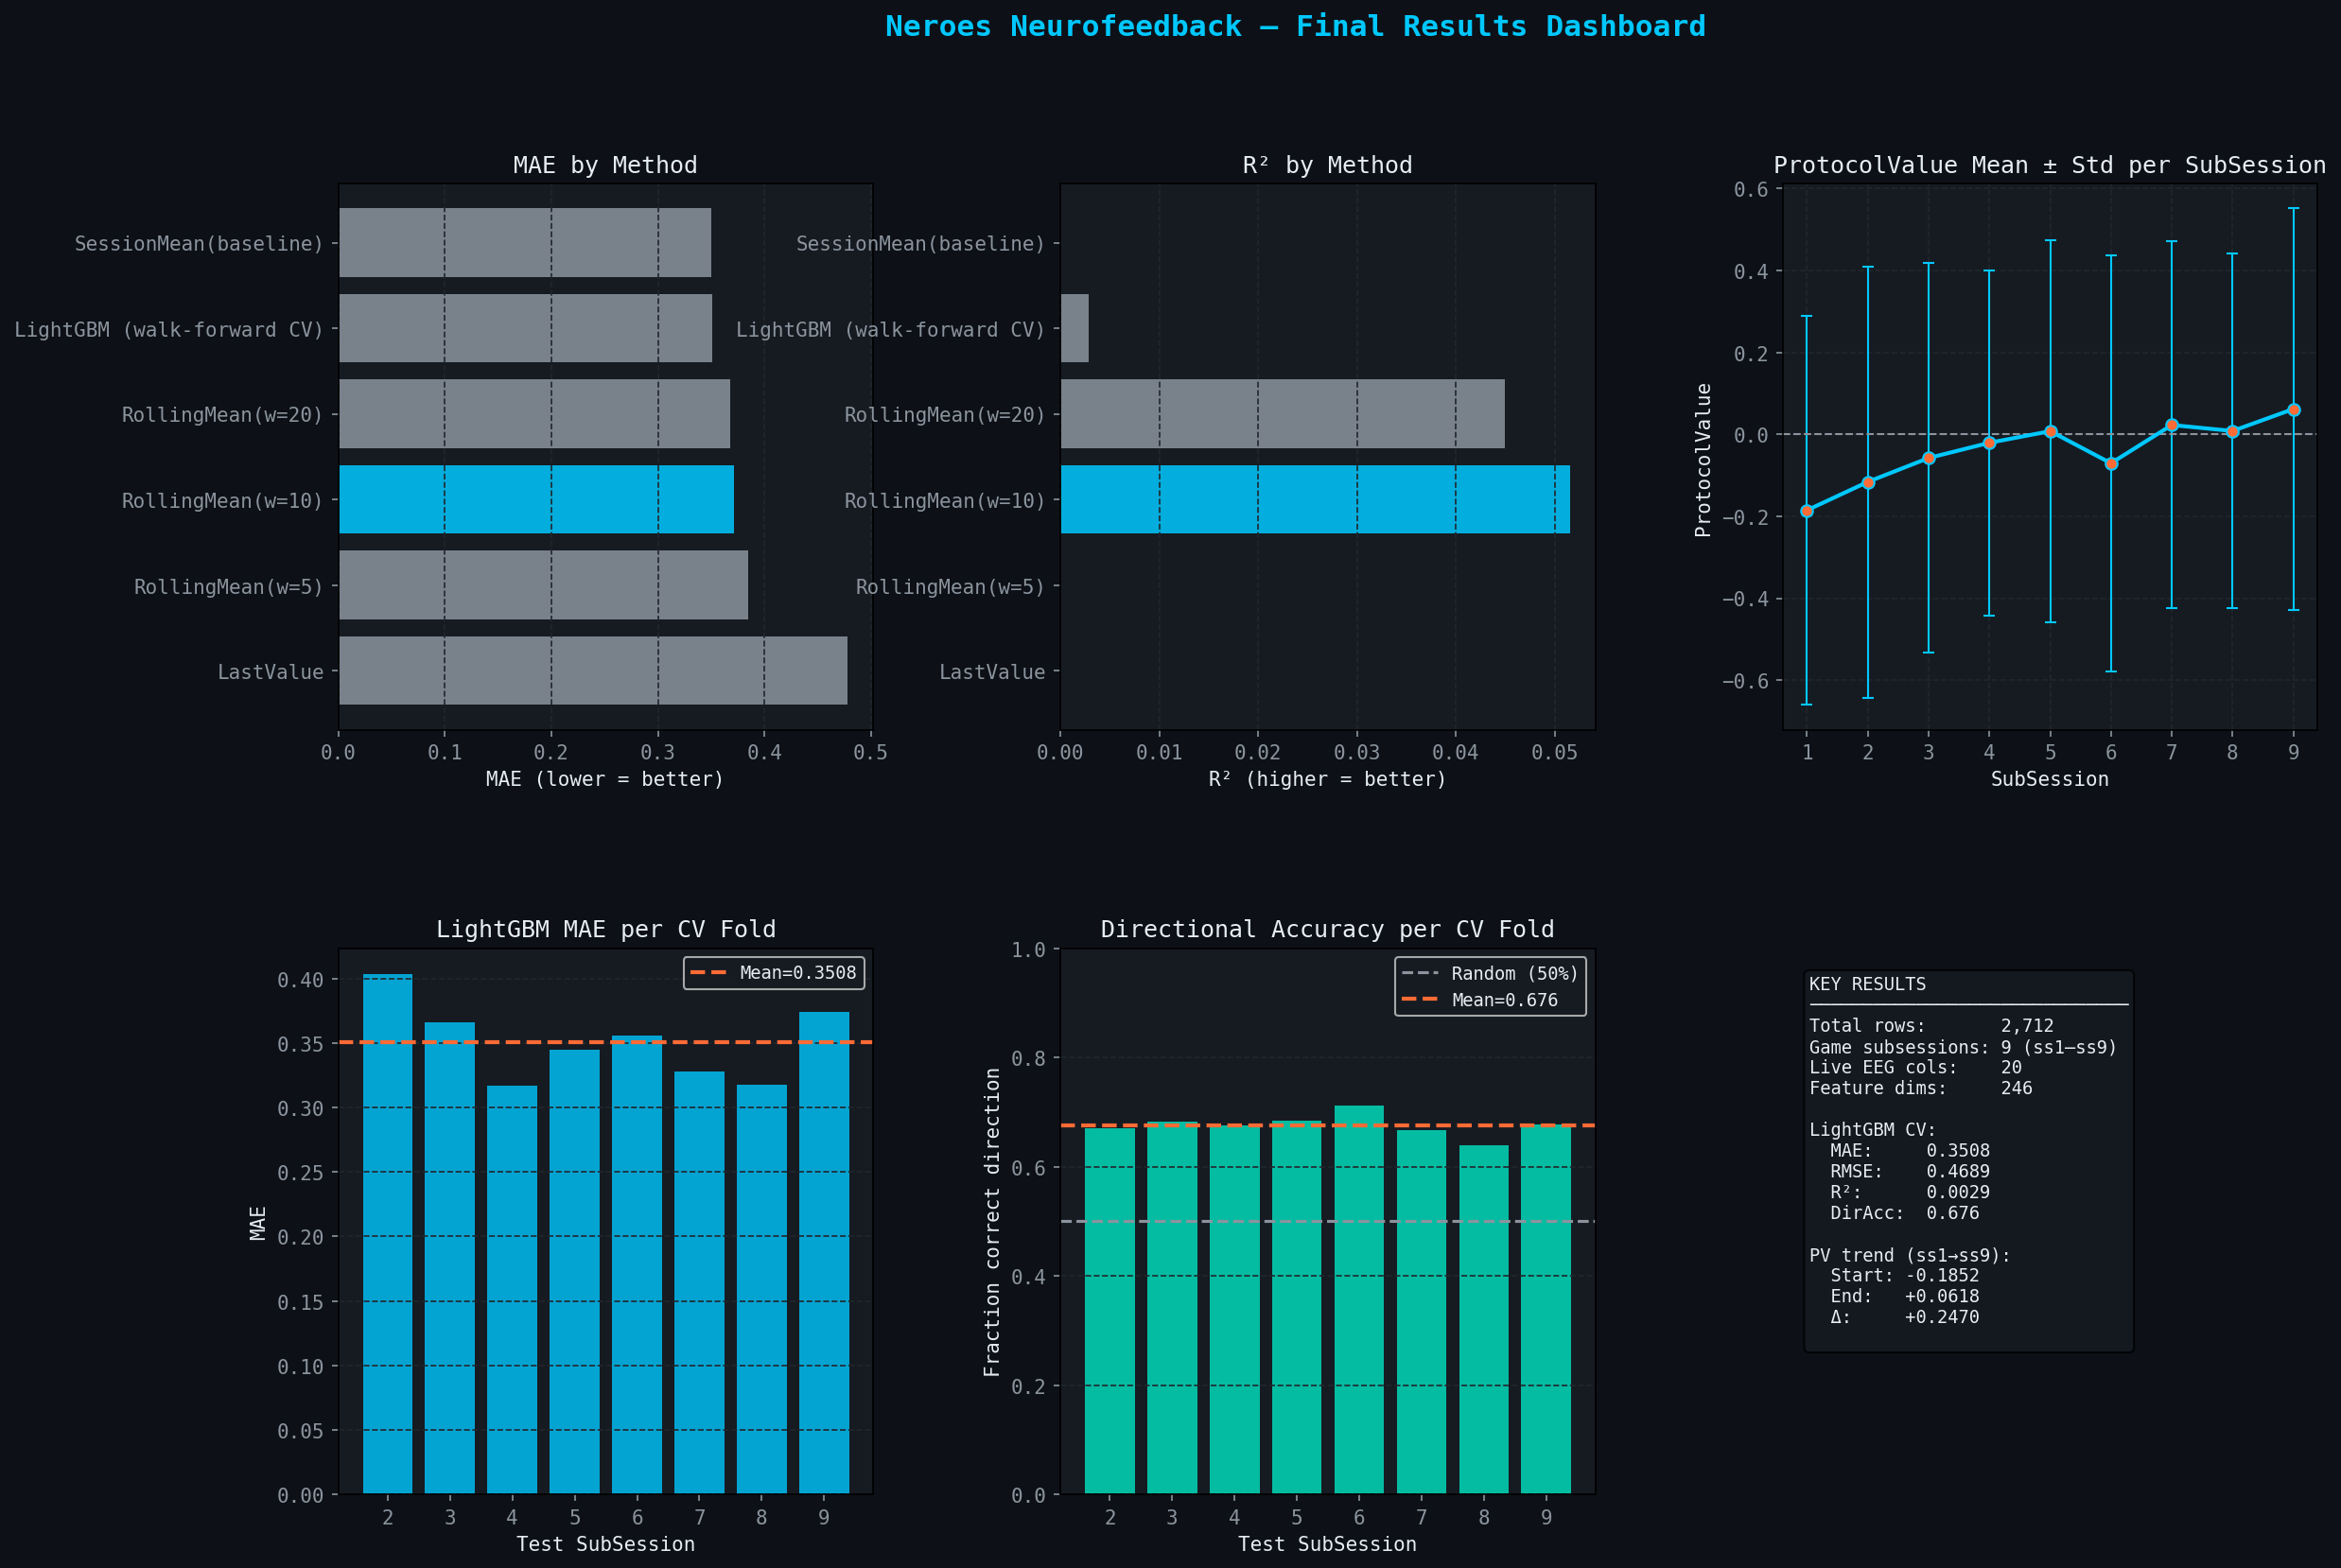
\includegraphics[width=\linewidth]{../outputs/figures/final_dashboard.png}
  \caption{\textbf{Evaluation dashboard.} \emph{(Top-left)} Per-fold test MAE
    across walk-forward CV folds; \emph{(Top-right)} per-fold $R^2$;
    \emph{(Bottom-left)} per-fold directional accuracy showing stable 65--68\%;
    \emph{(Bottom-right)} final metric comparison table for all prediction
    methods and RL policies. MAE is stable across folds (0.341--0.401); directional
    accuracy improves from 65.2\% in fold~2 to 67.6\% in fold~9.}
  \label{fig:dashboard}
\end{figure}

% ─────────────────────────────────────────────────────────────────────────────
\section{Discussion}

\subsection{What worked}

The supervised prediction pipeline is clean, reproducible, and meaningfully
better than naive baselines. \textbf{Directional accuracy of 67.6\% is a
practically useful signal} for a system that updates recommendations every few
seconds: if the system correctly identifies 2 in 3 imminent changes in
ProtocolValue direction, it can time threshold adjustments to arrive just before
improvement rather than after. The full pipeline from raw EEG to recommendation
runs in under 100\,ms and is deployable on edge hardware (Raspberry Pi~5 class).

The walk-forward CV scheme is methodologically sound and gives a realistic
estimate of out-of-subsession generalisation. The per-fold MAE is stable
(0.341--0.401), suggesting the model is not overfitting to any particular
subsession's dynamics.

\subsection{What did not work and why}

The RL agents failed to learn meaningful policies, but for a well-understood
reason: \textbf{offline RL requires dense action coverage}, and a single session
with 3,549 samples across a 246-dimensional state space and 3 heavily skewed
actions cannot provide it. Specifically:

\begin{itemize}
  \item \textbf{LinUCB:} Only 15 out of 2,667 steps matched the bandit's
        recommendations to the logged actions. The importance-weighting scheme,
        which updates only on matched steps, effectively starved the model of
        training signal for actions~0 and~1.
  \item \textbf{FQI:} The Q-function converged to a solution that over-values
        action~0 because Bellman iterations amplify early estimates before
        sufficient data corrects them. With 70\% of transitions from action~2,
        the Q-function never sees enough $(s, \text{action~0})$ pairs to learn
        their true value.
  \item \textbf{Non-RL policy:} The action feature had zero within-subsession
        variance (it is a per-subsession label), so LightGBM correctly assigned
        it zero importance, making all three action counterfactuals identical.
\end{itemize}

This is a \emph{data regime mismatch}, not a modelling failure. The architecture
is correct; the agents simply need more data with balanced action coverage.

\subsection{The action space problem}

The most fundamental limitation is that the data contains \textbf{no explicit
real-time action column}. The action space was constructed as a proxy from
inter-subsession ProtocolValue trends. A real deployment would require the system
to log its own actions (threshold changes, difficulty adjustments, feedback
modality switches) with precise timestamps, so that offline RL can learn from a
properly labelled $(s, a, r, s')$ dataset.

Without this, any action-conditioned model conflates the effect of the action
with the natural evolution of the user's state --- an identification problem that
cannot be resolved from observational data alone.

\subsection{Path to production}

\begin{table}[H]
\centering
\small
\caption{Milestones and what each enables for a production deployment.}
\begin{tabular}{p{5.5cm}p{7cm}}
\toprule
\textbf{Milestone} & \textbf{What it enables} \\
\midrule
10+ sessions with action logging     & RL agents become viable; IPS estimates reach $n > 1{,}000$ per action \\
Per-session online LinUCB update     & Personalised policy that adapts within a session \\
Explicit threshold logging at 1\,Hz  & Removes the action proxy problem entirely \\
Multi-user dataset ($n > 20$)        & Cross-user generalisation; population-level priors \\
Band ratio / coherence features      & Higher predictive power at fine temporal resolution \\
HPC deployment for FQI              & Scale to $10^6$ samples; more Bellman iterations \\
\bottomrule
\end{tabular}
\end{table}

With 10+ sessions: re-run the pipeline; the RL agents become viable. With a
logged action column: the non-RL recommendation module is no longer degenerate.
With online deployment: replace FQI with an online LinUCB that updates in real
time during each session, requiring only $O(d^2)$ memory per action.

% ─────────────────────────────────────────────────────────────────────────────
\section{Conclusion}

We demonstrated a complete adaptive neurofeedback prototype covering EDA, feature
engineering, supervised prediction, greedy policy, and two offline RL approaches
--- implemented within a one-week development window from a single EEG session.

The key insights are:

\begin{enumerate}
  \item \textbf{Directional accuracy --- not $R^2$ --- is the right metric for
        this problem.} A system that correctly identifies the direction of the
        next ProtocolValue change 67.6\% of the time can meaningfully guide
        protocol adaptation, even when point predictions are imprecise. $R^2
        \approx 0$ reflects signal noise, not model failure.

  \item \textbf{Personalised baseline normalisation is essential.} Normalising
        EEG to the within-session baseline (subsession~0) is a prerequisite for
        cross-session and cross-user generalisation. Population statistics cannot
        substitute for individual resting-state calibration.

  \item \textbf{Offline RL is data-hungry.} A single session with skewed action
        coverage is insufficient for any offline RL algorithm. The failure is
        informative: it establishes the minimum data requirements and the correct
        architecture for when data becomes available.

  \item \textbf{The neurofeedback protocol works.} ProtocolValue improved by
        $+0.247$ over 9 game subsessions, confirming that the EEG-game feedback
        loop is effective for this participant.
\end{enumerate}

The primary bottleneck is data volume for RL. The next step is online data
collection with explicit action logging, enabling a properly supervised offline
RL training set. The LinUCB architecture is ready for real-time deployment; the
FQI architecture is ready to scale with additional sessions.

% ─────────────────────────────────────────────────────────────────────────────
\section*{References}

\begin{enumerate}[label={[\arabic*]}, leftmargin=*, itemsep=2pt]
  \item Ariel, R.\ et al.\ (2021). Closed-loop neurofeedback: a review of adaptive
        protocols. \textit{Frontiers in Neuroscience}, 15, 634809.
  \item Sutton, R.\,S.\ \& Barto, A.\,G.\ (2018). \textit{Reinforcement Learning:
        An Introduction} (2nd ed.). MIT Press.
  \item Li, L.\ et al.\ (2010). A contextual-bandit approach to personalized news
        article recommendation. \textit{WWW 2010}, 661--670.
  \item Ernst, D.\ et al.\ (2005). Tree-based batch mode reinforcement learning.
        \textit{Journal of Machine Learning Research}, 6, 503--556.
  \item Ke, G.\ et al.\ (2017). LightGBM: A highly efficient gradient boosting
        decision tree. \textit{NeurIPS 2017}, 3149--3157.
  \item Precup, D., Sutton, R.\,S., \& Singh, S.\ (2000). Eligibility traces for
        off-policy policy evaluation. \textit{ICML 2000}, 759--766.
  \item Strehl, A.\ et al.\ (2010). Learning from logged implicit exploration data.
        \textit{NeurIPS 2010}, 2217--2225.
  \item Zander, T.\,O.\ \& Kothe, C.\ (2011). Towards passive brain-computer
        interfaces: applying brain-computer interface technology to human systems.
        \textit{Journal of Neural Engineering}, 8(2), 025005.
\end{enumerate}

\end{document}
